% !TEX program = xelatex
% 教學示例：一篇有「圖」也有「引用」的最小論文。
% 同一個專案要有三個檔：paper-with-figure.tex、practice.bib、figure-demo.pdf（由 figure-demo.gp 產生）。
% Overleaf：選 XeLaTeX 按 Recompile 即可（它會自動跑書目）。
% 本機：xelatex paper-with-figure → bibtex paper-with-figure → xelatex → xelatex（跑兩次，圖號與引用號才會對）。
\documentclass[11pt,a4paper]{article}
\usepackage{xeCJK}
\IfFontExistsTF{Microsoft JhengHei}{\setCJKmainfont{Microsoft JhengHei}}{\IfFontExistsTF{Songti TC}{\setCJKmainfont{Songti TC}}{\IfFontExistsTF{Noto Serif CJK TC}{\setCJKmainfont{Noto Serif CJK TC}}{\setCJKmainfont{FandolSong-Regular.otf}}}}
\usepackage[margin=2.5cm]{geometry}
\usepackage{graphicx}
\begin{document}
\title{論文工具箱練習：一張圖加一筆引用}
\author{你的稱呼（可用化名）}
\date{}
\maketitle

\section{我想了解的問題}
這份文件用來練習論文最常見的三件事：排版、放圖、引用。請把這段換成自己的研究問題。

\section{一張用 gnuplot 畫的圖}
圖~\ref{fig:errors} 是用 \texttt{figure-demo.gp} 讀 \texttt{figure-data.dat} 畫出來的示範資料，不是真實量測。
改資料檔再跑一次 gnuplot，重新編譯，這張圖就會跟著更新。

\begin{figure}[htbp]
  \centering
  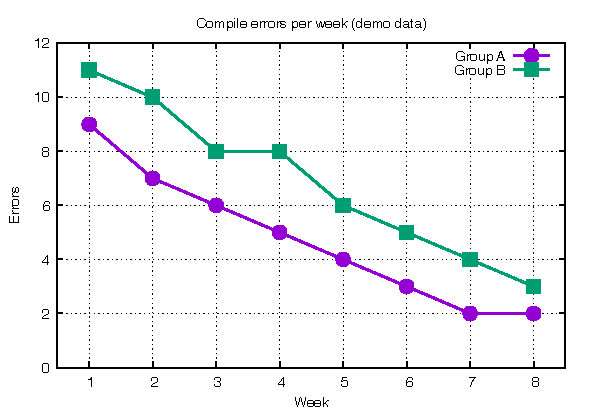
\includegraphics[width=0.8\linewidth]{figure-demo.pdf}
  \caption{每週編譯錯誤數（示範資料）。}
  \label{fig:errors}
\end{figure}

\section{一篇文獻}
Su 等人的研究於 2021 年刊登在 BMC Geriatrics \cite{Su2021}。
請回到原文核對題名、作者、年份和主張；這裡只示範引用怎麼接上書目檔。

\bibliographystyle{plain}
\bibliography{practice}
\end{document}
